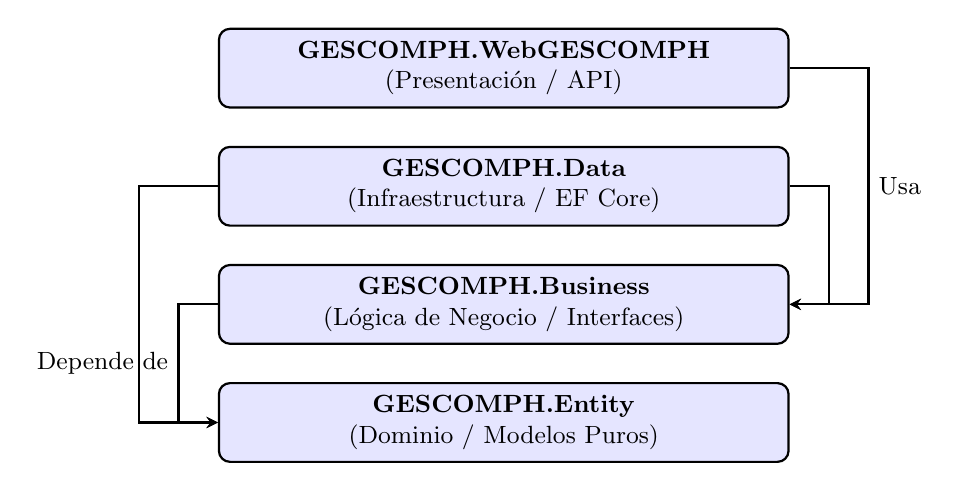
\begin{tikzpicture}[
    every node/.append style={font=\small},
    node distance=1.5cm, 
    auto,
    project/.style={rectangle, draw=black, thick, fill=blue!10, text width=7cm, align=center, minimum height=1cm, rounded corners},
    arrow/.style={thick, ->, >=stealth}
]
    % Nodos representando los proyectos
    \node[project] (web) {\textbf{GESCOMPH.WebGESCOMPH} \\ (Presentación / API)};
    \node[project, below of=web] (data) {\textbf{GESCOMPH.Data} \\ (Infraestructura / EF Core)};
    \node[project, below of=data] (business) {\textbf{GESCOMPH.Business} \\ (Lógica de Negocio / Interfaces)};
    \node[project, below of=business] (entity) {\textbf{GESCOMPH.Entity} \\ (Dominio / Modelos Puros)};

    % Flechas de dependencia
    \draw[arrow] (web.east) -- ++(1cm,0) |- (business.east) node[pos=0.25, right] {Usa};
    \draw[arrow] (data.east) -- ++(0.5cm,0) |- (business.east);
    \draw[arrow] (business.west) -- ++(-0.5cm,0) |- (entity.west) node[pos=0.25, left] {Depende de};
    \draw[arrow] (data.west) -- ++(-1cm,0) |- (entity.west);
    
    % Nota: Web también usa Data para inyección, pero arquitectónicamente pasa por Business
    % Simplificamos para claridad del diagrama
\end{tikzpicture}
